% ------------------------------------------------------------------------------
% TYPO3 Version 9.1 - What's New - Chapter "Changes for Integrators" (Serbian Version)
%
% @author	Michael Schams <schams.net>
% @license	Creative Commons BY-NC-SA 3.0
% @link		http://typo3.org/download/release-notes/whats-new/
% @language	English
% ------------------------------------------------------------------------------
% LTXE-CHAPTER-UID:		3a9852ea-e2360d9d-1ff5eec1-a7de3f9f
% LTXE-CHAPTER-NAME:	Changes for Integrators
% ------------------------------------------------------------------------------

\section{Izmene za integratore}
\begin{frame}[fragile]
	\frametitle{Izmene za integratore}

	\begin{center}\huge{Poglavlje 2:}\end{center}
	\begin{center}\huge{\color{typo3darkgrey}\textbf{Izmene za integratore}}\end{center}

\end{frame}

% ------------------------------------------------------------------------------
% LTXE-SLIDE-START
% LTXE-SLIDE-UID:		96df0292-243aea9f-1dc01b29-52f7f3ff
% LTXE-SLIDE-ORIGIN:	31b70474-edcc2a8a-d4a5fd3d-58734dc5 English
% LTXE-SLIDE-TITLE:		EXT:impexp - Maximum Number Of Records Restriction Removed
% LTXE-SLIDE-REFERENCE:	Deprecation-83592-ImpexpRemovedMaximumNumberOfRecordsRestriction
% ------------------------------------------------------------------------------

\begin{frame}[fragile]
	\frametitle{Izmene za integratore}
	\framesubtitle{Import/Export}

	Sistemsko prosirenje \texttt{impexp} je dozivelo brojna unapredjenja:

	\begin{itemize}
		\item Ogranicenje "maksimalan broj rekorda" je uklonjeno\newline
			\smaller
				Kada se eksportuju stranice ili rekordi, 
				ogranicenje za maksimalan broj rekorda je uklonjeno.
			\normalsize

		\item Ogranicenje "maksimalna velicina fajla" je uklonjeno\newline
			\smaller
				Prilikom eksporta fajlova koriscenjem "Export" interfejsa,
				ogranicenje da se eksportuju samo fajlovi odredjene velicine je uklonjeno.
			\normalsize

		\item Upravljanje velicinama je uklonjeno\newline
			\smaller
				Kada se eksportuju ili importuju strukture, rekordi i fajlovi
				upisivane su informacije o velicini fajlova za eksport i proveravale se tokom importa.
				Ova izmena ne utice na editore.
			\normalsize

	\end{itemize}

\end{frame}

% ------------------------------------------------------------------------------
% LTXE-SLIDE-START
% LTXE-SLIDE-UID:		83bfdb46-26e6908a-0fd6a9c6-df426142
% LTXE-SLIDE-ORIGIN:	0504ca33-7c23eff4-93a728fa-bd911c92 English
% LTXE-SLIDE-TITLE:		Redirect Functionality Moved To Redirects Module
% LTXE-SLIDE-REFERENCE:	83638-RedirectFunctionalityMovedFromSys_domainToRedirectsModule
% ------------------------------------------------------------------------------

\begin{frame}[fragile]
	\frametitle{Izmene za integratore}
	\framesubtitle{Funkcionalnost za redirekciju}

	\begin{itemize}
		\item Opcija da se konfigurise redirekcija kada se doda domen odredjenoj stranici ili grani je uklonjena.
		\item Redirekcije se sada mogu dodavati u novom modulu\newline
			\textbf{Site Management} \textrightarrow \textbf{Redirects}
	\end{itemize}

	\begin{figure}
		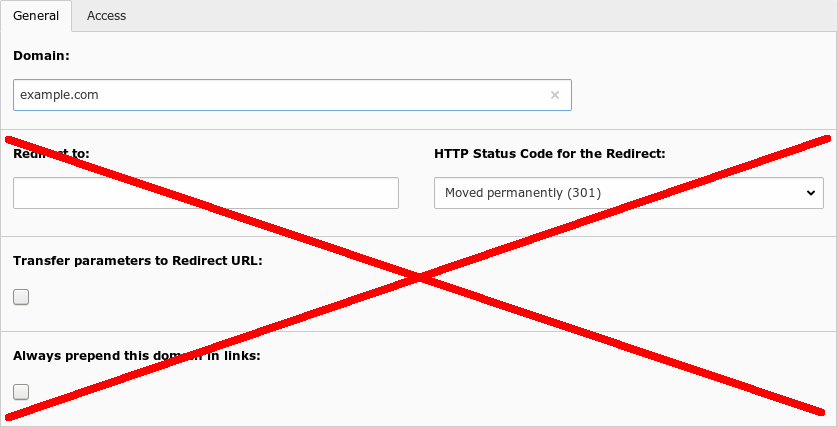
\includegraphics[width=0.6\linewidth]{ChangesForIntegrators/RedirectFunctionalityMovedToRedirectsModule.png}
	\end{figure}

\end{frame}

% ------------------------------------------------------------------------------
